\documentclass[12pt]{article}
\usepackage[top=1in, bottom=1in, left=1in, right=1in]{geometry}

\usepackage{setspace}
\onehalfspacing

\usepackage{amssymb}
%% The amsthm package provides extended theorem environments
\usepackage{amsthm}
\usepackage{epsfig}
\usepackage{times}
\renewcommand{\ttdefault}{cmtt}
\usepackage{amsmath}
\usepackage{graphicx} % for graphics files
\usepackage{tabu}

% Draw figures yourself
\usepackage{tikz} 

% writing elements
\usepackage{mhchem}

% The float package HAS to load before hyperref
\usepackage{float} % for psuedocode formatting
\usepackage{xspace}

% from Denovo Methods Manual
\usepackage{mathrsfs}
\usepackage[mathcal]{euscript}
\usepackage{color}
\usepackage{array}

\usepackage[pdftex]{hyperref}
\usepackage[parfill]{parskip}

% math syntax
\newcommand{\nth}{n\ensuremath{^{\text{th}}} }
\newcommand{\ve}[1]{\ensuremath{\mathbf{#1}}}
\newcommand{\Macro}{\ensuremath{\Sigma}}
\newcommand{\rvec}{\ensuremath{\vec{r}}}
\newcommand{\vecr}{\ensuremath{\vec{r}}}
\newcommand{\omvec}{\ensuremath{\hat{\Omega}}}
\newcommand{\vOmega}{\ensuremath{\hat{\Omega}}}
\newcommand{\sigs}{\ensuremath{\Sigma_s(\rvec,E'\rightarrow E,\omvec'\rightarrow\omvec)}}
\newcommand{\el}{\ensuremath{\ell}}
\newcommand{\sigso}{\ensuremath{\Sigma_{s,0}}}
\newcommand{\sigsi}{\ensuremath{\Sigma_{s,1}}}
%---------------------------------------------------------------------------
%---------------------------------------------------------------------------
\begin{document}
\begin{center}
{\bf NE 250, F15\\
November 2, 2015 
}
\end{center}

We've derived the Transport Equation, from it derived the Diffusion Equation, talked about the TE in the integral form, looked at the adjoint in detail, and quickly covered Monte Carlo methods. Finally, what about solving the integro-differential TE itself? That's next. We start with

The \textbf{Multigroup Approximation} (from L\&M 2.2)\\
We begin by setting up an energy grid, where $E_0$ is the highest energy value and $E_G$ is the lowest. We get $G-1$ groups and call the group between edge $g$ and edge $g-1$ group $g$. 

\begin{center}
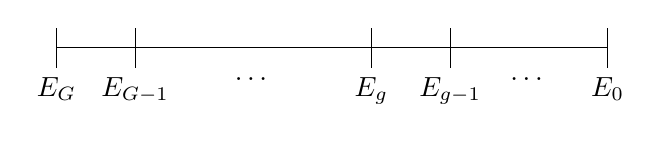
\begin{tikzpicture}
\draw (0,0)--(7,0);
\draw (0,-0.25)--(0, 0.25);
\draw (1,-0.25)--(1, 0.25);
\draw (4,-0.25)--(4, 0.25);
\draw (5,-0.25)--(5, 0.25);
\draw (7,-0.25)--(7, 0.25);
\node[below] at (0,-.25) {$E_G$};
\node[below] at (1,-.25) {$E_{G-1}$};
\node[below] at (2.5,-.25) {$\dots$};
\node[below] at (4,-.25) {$E_g$};
\node[below] at (5,-.25) {$E_{g-1}$};
\node[below] at (6,-.25) {$\dots$};
\node[below] at (7,-.25) {$E_0$};
\end{tikzpicture}
\end{center}

We use this grid to define the group flux
\[
\psi_g(\vecr, \vOmega) \equiv \int_{E_g}^{E_{g-1}} dE\: \psi(\vecr, \vOmega, E)
\]
Note that the continuous $\psi$ is in units of per eV, while the group angular flux is not, it includes all of the neutrons over that energy group. What we want to do next, is derive an equation whose solution is $\psi_g$, which means we will integrate the entire TE over energy. 

To perform that integral, we need to introduce an approximation. The one we will talk about now is \textit{assume the angular flux is separable in energy}:
\[
\psi(\vec{r}, \vOmega, E) \approx f(E)\psi_g(\vec{r}, \vOmega)\:, \quad E_g < E \leq E_{g-1}\:,
\]
where $f(E)$ is normalized such that $\int_g dE\: f(E) = 1$. We substitute and/or use this in the regular TE and integrate over energy. Here's how that works term by term.
%
%\begin{align*}
%\bigl[\vOmega \cdot \nabla + \Sigma_t\bigr] \psi(\vec{r}, E, \vOmega) &= \int_{4 \pi} d\vOmega' \int_0^{\infty} dE' \: \Sigma_s(E', \vOmega' \rightarrow E, \vOmega) \psi(\vec{r}, E', \vOmega')\\
% &+ \frac{\chi(E)}{4 \pi}\int_0^{\infty} dE' \: \nu(E') \Sigma_f(E') \int_{4 \pi} d\vOmega' \:\psi(\vec{r}, E', \vOmega')
%\end{align*}
\begin{itemize}
\item Streaming:
\[
\int_{E_g}^{E_{g-1}} dE\: \vOmega \cdot \nabla \psi(\vec{r}, \vOmega, E) = \vOmega \cdot \nabla \psi_g(\vec{r}, \vOmega)
\]

\item External (distributed fixed) source:
\[q_{g}(\vec{r}, \vOmega) \equiv \int_{E_g}^{E_{g-1}} dE\: q(\vec{r}, \vOmega, E)\]

\item Fission Source:
\begin{align*}
\int_{E_g}^{E_{g-1}} dE\: &\frac{\chi(E)}{4 \pi}\int_0^{\infty} dE' \: \nu(E') \Sigma_f(E') \int_{4 \pi} d\vOmega' \:\psi(\vec{r}, E', \vOmega') \\
&\chi_g \equiv \int_{E_g}^{E_{g-1}} dE\: \chi(E) \\
& \int_{4 \pi} d\vOmega' \:\psi(\vec{r}, E', \vOmega') = \phi(\vec{r}, E')\\
& \int_0^{\infty} dE' \: \nu(E') \Sigma_f(E') = \sum_{g'=1}^G \int_{E_g'}^{E_{g'-1}} dE'\: \nu(E') \Sigma_f(E')
\end{align*}
These second two items combine to form the fission source from group $g'$. We also need to define
\[
\nu\Sigma_{fg'} = \dfrac{\int_{E_g'}^{E_{g'-1}} dE'\: \nu(E') \Sigma_f(E')\phi(\vec{r}, E')}{\phi_{g'}(\vec{r})}
\]
and therefore the fission source in group $g$ is
\[
q_{fg} = \frac{\chi_g}{4 \pi}\sum_{g'=1}^G \nu\Sigma_{fg'} \phi_{g'}(\vec{r})
\]

\item Scattering term:
\end{itemize}



\end{document}
